\documentclass[border=1pt]{standalone}
\usepackage{tikz}
\usepackage{tikz-3dplot}

\begin{document}
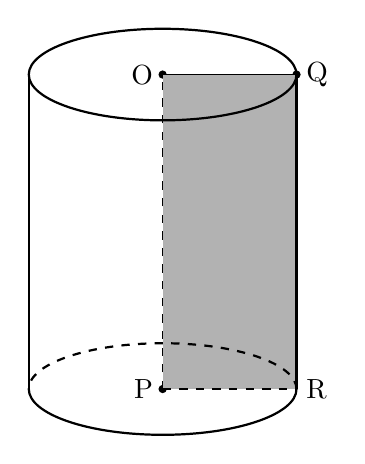
\begin{tikzpicture}
    \tdplotsetmaincoords{70}{0}
    \begin{scope}[tdplot_main_coords]
        
        % パラメータの定義
        \pgfmathsetmacro{\X}{3.4}
        \pgfmathsetmacro{\r}{\X/2}
        \pgfmathsetmacro{\h}{\X/4*5}
       
        % 頂点の座標の定義
        \coordinate (P) at (0,0,0); 
        \coordinate (O) at (0,0,\h); 
        \coordinate (R) at (\r,0,0);
        \coordinate (Q) at (\r,0,\h);
        \coordinate (T) at (-\r,0,0);
        \coordinate (S) at (-\r,0,\h);

        % 頂点のラベル
        \fill (P) circle (1.5pt) node[left] {$\mathrm{P}$};
        \fill (O) circle (1.5pt) node[left] {$\mathrm{O}$};
        \node[right] at (R) {$\mathrm{R}$};
        \fill (Q) circle (1.5pt) node[right] {$\mathrm{Q}$};  

        % 網掛け
        \fill[black!30] (P) rectangle (Q);

        % 線の描画
        \draw [thick,dashed] (R) arc (0:180:\r);
        \draw [thick] (R) arc (0:-180:\r);
        \draw [thick] (Q) arc (0:360:\r);
        \draw [semithick, dashed] (P) -- (O);
        \draw [thick] (R) -- (Q);
        \draw [thick] (T) -- (S);
        \draw [semithick, dashed] (P) -- (R);
        \draw [semithick] (O) -- (Q);
    
    \end{scope}
 
\end{tikzpicture}
\end{document}
